\documentclass{article}
\usepackage{tikz}
\usetikzlibrary{calc}

\begin{document}

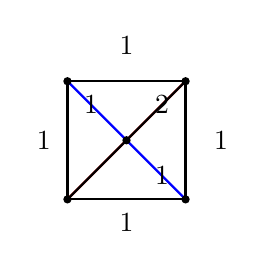
\begin{tikzpicture}[scale=1.5]
    % Define coordinates for the vertices
    \coordinate (A) at (0,0);
    \coordinate (B) at (1,0);
    \coordinate (C) at (1,1);
    \coordinate (D) at (0,1);
    \coordinate (E) at (0.5,0.5);

    % Draw the square
    \draw[thick] (A) -- (B) -- (C) -- (D) -- cycle;
    
    % Draw the red line representing slice S
    \draw[thick, color=red] (A) -- (E) -- (C);
    
    % Draw the blue line representing slice T
    \draw[thick, color=blue] (B) -- (E) -- (D);
    
    % Draw the diagonal line
    \draw[thick] (A) -- (C);
    
    % Label the edges
    \node at (0.5,-0.2) {$1$};
    \node at (1.3,0.5) {$1$};
    \node at (-0.2,0.5) {$1$};
    \node at (0.5,1.3) {$1$};
    \node at (0.8,0.2) {$1$};
    \node at (0.2,0.8) {$1$};
    \node at (0.8,0.8) {$2$};
    
    % Mark the vertices
    \fill (A) circle (1pt);
    \fill (B) circle (1pt);
    \fill (C) circle (1pt);
    \fill (D) circle (1pt);
    \fill (E) circle (1pt);
\end{tikzpicture}

\captionof{figure}{Two adjacent, troublesome slices: A 4-matching on \( W_5 \) containing two full-index troublesome slices, \( S \) (in \textcolor{red}{red}) and \( T \) (in \textcolor{blue}{blue}), that are somewhat, but not almost disjoint. Notice that our algorithm can choose either the outer edge of \( S \) or the outer edge of \( T \), but not both.}
\end{document}